%%%%%%%%%%%%%%%%%%%%%%%%%%%%%%%%%%%%%%%%%%%%%%%%%%%%%%%%%%%%%%%%%%%%%%%%%%%%%%%%%%%%%%%%%%%%%%%%%%%%%%%%%%%%%%%%%%%%%%%%%%%%%%%%%%%%%%%%%%%%%%%%%%%%%%%%%%%
% This is just an example/guide for you to refer to when submitting manuscripts to Frontiers, it is not mandatory to use Frontiers .cls files nor frontiers.tex  %
% This will only generate the Manuscript, the final article will be typeset by Frontiers after acceptance.   
%                                              %
%                                                                                                                                                         %
% When submitting your files, remember to upload this *tex file, the pdf generated with it, the *bib file (if bibliography is not within the *tex) and all the figures.
%%%%%%%%%%%%%%%%%%%%%%%%%%%%%%%%%%%%%%%%%%%%%%%%%%%%%%%%%%%%%%%%%%%%%%%%%%%%%%%%%%%%%%%%%%%%%%%%%%%%%%%%%%%%%%%%%%%%%%%%%%%%%%%%%%%%%%%%%%%%%%%%%%%%%%%%%%%

%%% Version 3.4 Generated 2018/06/15 %%%
%%% You will need to have the following packages installed: datetime, fmtcount, etoolbox, fcprefix, which are normally inlcuded in WinEdt. %%%
%%% In http://www.ctan.org/ you can find the packages and how to install them, if necessary. %%%
%%%  NB logo1.jpg is required in the path in order to correctly compile front page header %%%

\documentclass[utf8]{frontiersSCNS} 
\usepackage{url,hyperref,lineno,microtype,subcaption,natbib}
\usepackage[onehalfspacing]{setspace}
\usepackage[english]{babel}
\usepackage{changes}
\definechangesauthor[name={George Chack}, color=orange]{gc}
%\setremarkmarkup{(#2:#1)}
%\linenumbers
\usepackage{amsmath}

% Leave a blank line between paragraphs instead of using \\

\def\keyFont{\fontsize{8}{11}\helveticabold }
\def\firstAuthorLast{Zhao {et~al.}} %use et al only if is more than 1 author
\def\Authors{Wenxi Zhao\,$^{1}$ and George Chacko\,$^{1,*}$} %Co-Author\,$^{2}$ 
% Affiliations should be keyed to the author's name with superscript numbers and be listed as follows: Laboratory, Institute, Department, Organization, City, State abbreviation (USA, Canada, Australia), and Country (without detailed address information such as city zip codes or street names).
% If one of the authors has a change of address, list the new address below the correspondence details using a superscript symbol and use the same symbol to indicate the author in the author list.
\def\Address{$^{1}$Netelabs, NET ESolutions (an NTT DATA Company), McLean, VA, USA}

% The Corresponding Author should be marked with an asterisk
% Provide the exact contact address (this time including street name and city zip code) and email of the corresponding author
\def\corrAuthor{George Chacko}

\def\corrEmail{netelabs@nete.com}
\begin{document}
\onecolumn
\firstpage{1}

\title[Running Title]{Placeholder: Delayed Recognition of Co-cited Articles} 

\author[\firstAuthorLast ]{\Authors} %This field will be automatically populated
\address{} %This field will be automatically populated
\correspondance{} %This field will be automatically populated

\extraAuth{}% If there are more than 1 corresponding author, comment this line and uncomment the next one.
%\extraAuth{corresponding Author2 \\ Laboratory X2, Institute X2, Department X2, Organization X2, Street X2, City X2 , State XX2 (only USA, Canada and Australia), Zip Code2, X2 Country X2, email2@uni2.edu}

\maketitle

% ABSTRACT
\begin{abstract}
Enter abstract text later
\end{abstract}

\section{Introduction}

\replaced[id=gc]{The term `Sleeping Beauty' has been used to describe an article that is not well cited in the early years after its publication but experiences a sharp increase in the rate at which it is subsequently cited~\citep{Raan2004}. An implication is that the discovery reported in such an article is `ahead of its time' and recognition is delayed. Causes have been postulated that include information overload on account of the large amount of information available, the communication skills of authors, insufficient promotion of ideas, conflict with existing theory and experimental data, the author's position in the social hierarchy of science, multiple discovery, the extent to which scientific institutions are established and organized, the conservative nature of the establishment and other reasons for resistance~\citep{Barber1961,Merton1963,Cole1970,Garfield1970a,Garfield1980a}. The phenomenon (and its Sleeping Beauty label) has been further discussed, studied and quantified with varying definitions but some agreement that a fraction of the scientific literature exhibits citation kinetics that suggest delayed recognition of a new idea~\citep{Glanzel2003,Glanzel2004,Braun_2010,Li2014,Ke2015,Li2016,Song2018,sugimoto_mostafa_2018} .


New ideas may also result from combining two previously independent ones and such events can be traced through co-citation analysis~\citep{MarshakovaShaikevich1973,Small1973}. The initial definition of co-citation independently by Marshakova-Shaikevich and Small in 1973 has been followed up by a number of studies that examine novelty from different perspectives of co-citation~\citep{Uzzi2013,Boyack2014,Wang2017,Bradley2020}. In another study on co-citation, we used simple criteria to identify instances of co-cited articles with delayed kinetics, which we termed delayed co-citations [Devarakonda et al.]. 

In this article, we extend observations on delayed co-citations by applying criteria modified from the scale-free beauty coefficient formulation~\citep{Ke2015} as well as the approach of Raan~\citep{Raan2004,Raan2019}. \emph{We need to read the Fred Ye papers as well as Wang}. Using a dataset of approximately 4.12 million co-cited pairs, we do x,y, and z.}{Sleeping Beauty in scientific community refers to a single well-cited article which receives delayed recognition because of being ahead of time or overlooked for periods. Anthony F.J. van Raan and other researchers have proposed different methods to identify Sleeping Beauty articles and measure their kinetics. This phenomenon also happens for co-cited pairs that a pair of publications have been cited by one or more publications together. The more often a pair of publications has been co-cited, the more related they are assumed to be https://arxiv.org/pdf/1707.03076.pdf. The appearance of Sleeping Beauty among co-cited pairs indicates that as time goes on, different disciplines gradually have overlaps or different ideas have been combined and evolved into a new concept. In our experiment, we extend to examine Sleeping Beauty phenomenon for highly co-cited pairs that have been sunk in sleep for a long period before attracting citations, propose an approach to define Sleeping Beauty among co-cited pairs and investigate the kinetics of Sleeping Beauty co-cited pairs and their individual articles. To find possible Sleeping Beauty co-cited pairs, we constructed a dataset of articles from Scopus (Elsevier BV, 2019) by extracting co-cited pairs which were composed of highly co-cited individual articles and have received at least 10 co-citations. We assembled 4.12 million co-cited pairs as a result. We developed an initial method to find possible Sleeping Beauty co-cited pairs within our dataset, and in order to further investigate kinetics of those possible Sleeping Beauty co-cited pairs, we built another dataset of individual articles from filtered co-cited pairs. To determine the number of Sleeping Beauty individual articles found in this dataset, we applied modified van Raan's procedures to filter out articles by setting the most stringent constraints and then calculated the beauty coefficient proposed by Ke et al. Then by calculating the number of Sleeping Beauty individual articles that each filtered co-cited pairs has and adjusting the constraints we applied, we answered the question that does it take at least one Sleeping Beauty individual article to generate a Sleeping Beauty co-cited pair. Lastly, we also investigated edge cases that a co-cited pair awaked after a long period of dormancy and then fell asleep again. We proposed a new method to define such Sleeping Beauty individual articles, since both van Raan's and Ke's method were not applicable in such cases, and defined them as unstable Sleeping Beauties.}

 

\iffalse
 Sleeping Beauty in scientific community refers to a single well-cited article which receives delayed recognition because of being ahead of time or overlooked for periods. Anthony F.J. van Raan and other researchers have proposed different methods to identify Sleeping Beauty articles and measure their kinetics. This phenomenon also happens for co-cited pairs that a pair of publications have been cited by one or more publications together. The more often a pair of publications has been co-cited, the more related they are assumed to be \footnote{https://arxiv.org/pdf/1707.03076.pdf}. The appearance of Sleeping Beauty among co-cited pairs indicates that as time goes on, different disciplines gradually have overlaps or different ideas have been combined and evolved into a new concept. In our experiment, we extend to examine Sleeping Beauty phenomenon for highly co-cited pairs that have been sunk in sleep for a long period before attracting citations, propose an approach to define Sleeping Beauty among co-cited pairs and investigate the kinetics of Sleeping Beauty co-cited pairs and their individual articles. 

To find possible Sleeping Beauty co-cited pairs, we constructed a dataset of articles from Scopus (Elsevier BV, 2019) by extracting co-cited pairs which were composed of highly co-cited individual articles and have received at least $10$ co-citations. We assembled $4.12$ million co-cited pairs as a result.

We developed an initial method to find possible Sleeping Beauty co-cited pairs within our dataset, and in order to further investigate kinetics of those possible Sleeping Beauty co-cited pairs, we built another dataset of individual articles from filtered co-cited pairs. To determine the number of Sleeping Beauty individual articles found in this dataset, we applied modified van Raan's procedures to filter out articles by setting the most stringent constraints and then calculated the beauty coefficient proposed by Ke et al. Then by calculating the number of Sleeping Beauty individual articles that each filtered co-cited pairs has and adjusting the constraints we applied, we answered the question that does it take at least one Sleeping Beauty individual article to generate a Sleeping Beauty co-cited pair. 

Lastly, we also investigated edge cases that a co-cited pair awaked after a long period of dormancy and then fell asleep again. We proposed a new method to define such Sleeping Beauty individual articles, since both van Raan's and Ke's method were not applicable in such cases, and defined them as unstable Sleeping Beauties.
\fi


\section{MATERIAL AND METHODS}



[process of getting 4.12 million data]


To find possible sleeping beauty pairs, we set four stringent conditions on $4.12$ million co-cited pairs: (1) The total number of co-citation frequency that a co-cited pair received is at least $100$; (2) The highest co-citation frequency that a co-cited pair received is at least $20$; (3) Both individual papers for a co-cited pair should have published no earlier than $1970$; (4) A co-cited paper should have slept for at least $10$ years and received no more than $2$ co-citations in each year during sleeping period. 
The sleeping duration for a co-cited pair is defined as the number of years from the first possible co-cited year, which is the publication year of the newer individual paper, to the first year that the pair receives more than $2$ co-citations. $1380$ co-cited pairs satisfy have been extracted from $4.12$ million pairs data and have been labeled as possible sleeping beauty co-citation pairs for further experiment. 
Next, we used a parameter-free approach, proposed by~\citep{Ke2015}, and a bibliometric approach, proposed by~\citep{Raan2019}, to investigate whether the individual papers of $1380$ co-cited pairs are sleeping beauties or not. 

Ke et al proposed Beauty Coefficient B to quantify how much a given paper can be considered as an SB~\citep{Ke2015}. Given a publication, Ke defines $c\textsubscript{0}$ as the number of citations received in the year of publication and $c\textsubscript{t}$ as the number of citations received in each year after the year of publication, where $t$ indicates the number of years. The reference line of a publication is defined as a straight line $l\textsubscript{t}$ that connects the start point $(0, c\textsubscript{0})$ and peak point $(t\textsubscript{m}, c\textsubscript{t\textsubscript{m}})$ where $m$ indicates that at the age of $t\textsubscript{m}$ the paper receives its maximum number of citations $c\textsubscript{t\textsubscript{m}}$. Then this line $l\textsubscript{t}$ can be described by the equation:
\begin{equation}
\l\textsubscript{t} = \frac{c\textsubscript{t\textsubscript{m}} - c\textsubscript{0}}{t\textsubscript{m}} \times t + c\textsubscript{0}
\end{equation}
where $t \in [t\textsubscript{0}, t\textsubscript{m}]$ and ${c\textsubscript{t\textsubscript{m}} - c\textsubscript{0}}/{t\textsubscript{m}}$ is the slope of the reference line. Then for each $t$, first compute difference between the reference line l\textsubscript{t} and the citation history of the paper c\textsubscript{t}, and second compute the ratio between this difference and $max\{1, c\textsubscript{t}\}$. By summing up this ratio for each $t$, the Beauty Coefficient B is defined as:
\begin{equation}
B = \sum_{t = 0}^{t\textsubscript{m}} \frac{\frac{c\textsubscript{t\textsubscript{m}} - c\textsubscript{0}}{t\textsubscript{m}} \times t + c\textsubscript{0} - c\textsubscript{t}}{max\{1, c\textsubscript{t}\}}
\end{equation}

\begin{figure}
\begin{center}
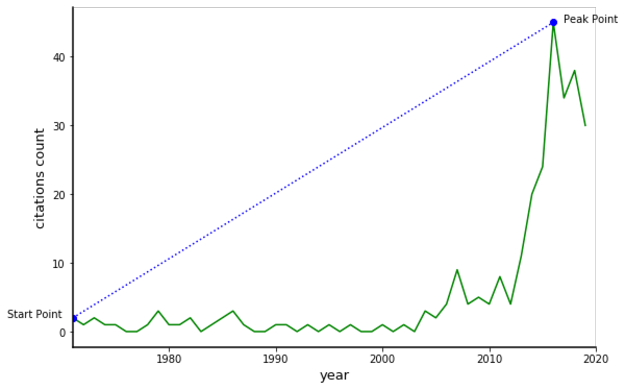
\includegraphics{Picture1}
\caption{Demonstration of Ke's Beauty Coefficient (Eq. 2)}\label{fig:1} 
\end{center}
(We can discuss whether we should add anything to this plot based on the defects I stated below, or cite it directly from Ke, or just remove it)
\end{figure}

On  \textbf{Figure 1}, The green curve represents the number of citations c\textsubscript{t}that a paper received at each year and $t$ is the number of years between two years. The blue dotted line represents the reference line, which connects the peak point $(t\textsubscript{m}, c\textsubscript{t\textsubscript{m}})$ and start point $(0, c\textsubscript{0})$. This Beauty Coefficient B can be computed for any paper and does not rely on arbitrary selections of parameters such as length of sleeping period and awakening intensity. A paper who have a linear kinetics with time $c\textsubscript{t} = l\textsubscript{t}$ will have Beauty Coefficient $B = 0$, and thus if a paper can be considered as Sleeping Beauty, it must have a positive Beauty Coefficient, which means its kinetics is a concave function of time. Further, this equation penalizes earlier citations since the summation of ratio in earlier years will be much less than the one in later years when the number of citations received is the same, and so with longer sleeping period, larger maximum citations received, and more abrupt changes happened before the maximum number of citations reached, a publication will have a larger Beauty Coefficient B. 

But Ke's method also has three major defects: (i) This approach doesn't put any constraints on any parameters. In general, a paper who has very large Beauty Coefficient B will have a long sleeping period, abrupt changes in citations received before reaching the peak point, and a very high peak point. But in extreme cases, as long as the peak point is high enough, a paper will definitely have a larger B value. For example, if a paper published in $2014$ receives $3000$ citations in $2018$, then even though the sleeping period is only $3$ years and each year receives only $2$ citations, by (Eq. 2) the Beauty Coefficient B equals to $2998$, which is large enough for a paper to be identified as Sleeping Beauty(Ke et al lists top 15 Sleeping Beauties in science and all of those papers have Beauty Coefficient B larger than 2000~\citep{Ke2015}). The paper in such extreme case apparently shouldn't be considered as Sleeping Beauty, which also proves that a paper must have a large positive Beauty Coefficient to be identified as Sleeping Beauty, but a paper with large positive Beauty Coefficient is not necessarily a Sleeping Beauty. (ii) Ke et al mentions that Sleeping Beauty papers will have a large Beauty Coefficient B, but he doesn't provide a exact threshold to define how large a Beauty Coefficient B should a paper have to be a Sleeping Beauty. When he examines interdisciplinary nature of top Sleeping Beauties, he divides papers into three disjoint subsets with high, medium, and low values of Beauty Coefficient B, which is the group of top $1000$ SBs $(B \geq 317.93)$, the $1001st$ to the top $1\%$ SBs $(33.21 \leq B \leq 317.93)$, and the rest $(B \leq 33.21)$~\citep{Ke2015}). These cutoff values are quite arbitrary and cannot be directly applied to other datasets. Thus the application of this Beauty Coefficient is quite unclear. (iii) Ke et al does not consider the citations received after the peak point is reached. Since Sleeping Beauty papers are those who have delayed recognization, in most cases they will keep sleeping in earlier years, gradually gain citations and reach the peak point in recent years. But this doesn't mean that we can completely ignore the kinetics after the peak point is reached. The biggest problem it will cause is that when a paper reaches its peak point twice, how should this reference line be drawn? Should we connect the start point to the first peak point or the second peak point? What if there are more than two peaks? Further, if a paper reaches its peak point in its publication year, and goes back to sleep for several years and wake up again, should we ignore all those kinetics since the start point equals to the peak point and the reference line could not be drawn? We'll further explore this kine of edge case later. 

van Raan proposed another totally different method to identify Sleeping Beauties. He tuned four main parameters: (1) length of sleeping period; (2) depth of sleep, in terms of the citation rate during sleeping period; (3) awakening period, which is $5$ years after sleeping period; (4) awakening citation-intensity in terms of the citation rate during awakening period~\citep{Raan2019}). van Raan focused on investigating the number of SBs identified with different combinations of parameters, especially with different length of sleeping period, and deriving the general 'General Sleeping Beauty Equation' to gives the number of SBs identified depend on those parameters. 

In our experiment, we made minor adjustments to this method. Based on initial limitations we set on our Sleeping Beauty co-citation pairs, we also required individual papers to have slept for at least $10$ years. Thus we didn't split sleeping period into several classes as van Raan did, instead we calculated the exact length of sleeping duration for each paper. After adjustments, we also have four main parameters as van Raan proposed and the corresponding limitations are: (1) the length of sleeping period should be at least $10$ years; (2) the citation rate during sleeping period should be between $0$ and $1$; (3) the awakening period is defined as $5$ years following the sleeping period; (4) the citation rate during awakening period should be at least $5$. Given that $t\textsubscript{0}$ is the year of publication, $t\textsubscript{n}$ is the last year of sleeping duration and $c\textsubscript{$t\textsubscript{i}$}$ is the number of citations received at year $t\textsubscript{i}$, the definition of Sleeping Beauty can be written out as:
\begin{equation}
\text{for }\ n \geq 10, 0 \leq \{c\textsubscript{t\textsubscript{0}} + ... + c\textsubscript{t\textsubscript{n}}\}/n \leq 1, \{c\textsubscript{t\textsubscript{n+1}} + ... + c\textsubscript{t\textsubscript{n+5}}\}/5 \geq 5
\end{equation}
Although van Raan's method is very solid, we still find that one thing has been overlooked: since van Raan didn't consider the maximum number of citations received as an important parameter to be tuned, in cases where a paper slept for ten years, has citation rate during sleeping period between $0$ and $1$, and then has received $5$ citations each year for $5$ years, which is the awakening period, it shouldn't be identified as a Sleeping Beauty. In such case, the paper satisfies all conditions but it doesn't show an increasing trend during awaking period. Further, after the awaking period, the paper can go back to sleep again. In such case, this paper will reach its peak point, $5$ citations, in its awaking period. van Raan didn't specify either the peak point can't be reached during awaking period or the minimum value of peak point, and this will mistakenly identify some unqualified papers as Sleeping Beauty.

From our $1380$ Sleeping Beauty co-cited pairs, we generated the dataset of $1398$ individual publications. To identify Sleeping Beauties from this dataset, we used Ke's and van Raan's method to identify SBs independently and compare the result, and then combined them together to avoid some defects mentioned before. Right now we only consider individual publications that have only one peak point. By applying both methods independently, we got the result of number of SBs identified in this $1398$ individual publications dataset. Further, we extracted out Sleeping Beauty co-citation pairs which have at least one individual publication is identified as SB. Then by comparing the result of number of SBs identified by both methods and the number of pairs that have at least one SB, we found the overlaps and difference between two methods, which helped us design the next experiment to combine two methods together.

After setting limitations on individual publications based on van Raan's paper to extract possible SBs, we calculated Beauty Coefficient for those SBs. Then we designed an experiment to calculate the minimum number of Beauty Coefficient that a paper should have and set it as threshold for us to filter out qualified SBs. By setting van Raan's conditions first, papers that have (1) sleeping duration is at least $10$ years; (2) citation rate during sleeping duration is between $0$ and $1$; (3) citation rate during awakening period is at least 5; (4) the maximum number of citations received is at least 20; will be extracted out. Thus we avoided the first defect that Ke's method has and the overlooked point of van Raan's method by setting the peak point. For an extreme case, the minimum conditions that a a paper should have are listed below:
\begin{equation}
n = 10,  \{c\textsubscript{t\textsubscript{0}} + ... + c\textsubscript{t\textsubscript{n}}\}/n = 1, \{c\textsubscript{t\textsubscript{n+1}} + ... + c\textsubscript{t\textsubscript{n+5}}\}/5 = 5, c\textsubscript{t\textsubscript{m}} \geq 20
\end{equation}
where c\textsubscript{t\textsubscript{m}} is the maximum number of citations received, which means at year t\textsubscript{m} the paper reaches its peak point. 

[Implement algorithm to find threshold here]

[Edge case: papers that have more than one peak point. I'm still working on how to measure this kind of edge case. A plot will be added here]


\section{RESULT AND DISCUSSION}

As we mentioned above, by setting four stringent conditions on our $4.12$ million pairs data, we extracted out $1380$ Sleeping Beaut y co-citation pairs. To investigate the relationship between Sleeping Beauty co-citation pairs and Sleeping Beauty individual publications, we further explored kinetics of $1398$ individual papers which composed of our $1380$ Sleeping Beauty co-citation pairs dataset. By using both parameter-free approach and parameter-dependent approach, which are proposed by Ke et al and van Raan respectively, we got $123$ Sleeping Beauty individual publications identified by van Raan's method, and since Ke didn't set a clear threshold for Beauty Coefficient, we set different threshold by adjusting the quantile of Beauty Coefficient and extracted out papers that have Beauty Coefficient higher than each threshold. Next, we recorded the number of papers that have been identified as Sleeping Beauty by both Ke and van Raan, and got the number of Sleeping Beauty co-citation pairs that have at least $1$ SB, have $2$ SBs, and have $0$ SB. The results shows in the following table:
\begin{table}[ht]
\caption{Result Table} % title of Table
\centering % used for centering table
\begin{center}
\begin{tabular}{c c c c c c c} % centered columns (4 columns)
B Threshold & B Value & \#SB by Ke & \#SB by Both & \#Pairs with SB=0 & \#Pairs with SB=1 & \#Pairs with SB=2 \\ [0.5ex] % inserts table
%heading
\hline % inserts single horizontal line
$\geq$1000 & 1000 & 30 & 12 & 1358 & 20 & 2 \\ % inserting body of the table
0.90 quantile & 336.64 &140 & 42 & 1308 & 65 & 7 \\
0.75 quantile & 177.79 & 350 & 61 & 1260 & 105 & 15 \\
0.50 quantile & 82.11 & 699 & 114 & 1229 & 129 & 22 \\
0.25 quantile & 37.37 & 1408 & 123 & 1220 & 137 & 23 \\ [1ex] % [1ex] adds vertical space
\hline %inserts single line
\end{tabular}
\end{center}
\label{table:nonlin} % is used to refer this table in the text
\end{table}


\section{CONCLUSION}

[Add Conclusions Here]


\section{Additional Requirements}

For additional requirements for specific article types and further information please refer to \href{http://www.frontiersin.org/about/AuthorGuidelines#AdditionalRequirements}{Author Guidelines}.

\section*{Conflict of Interest Statement}
%All financial, commercial or other relationships that might be perceived by the academic community as representing a potential conflict of interest must be disclosed. If no such relationship exists, authors will be asked to confirm the following statement: 

The authors declare that the research was conducted in the absence of any commercial or financial relationships that could be construed as a potential conflict of interest.

\section*{Author Contributions}

The Author Contributions section is mandatory for all articles, including articles by sole authors. If an appropriate statement is not provided on submission, a standard one will be inserted during the production process. The Author Contributions statement must describe the contributions of individual authors referred to by their initials and, in doing so, all authors agree to be accountable for the content of the work. Please see  \href{http://home.frontiersin.org/about/author-guidelines#AuthorandContributors}{here} for full authorship criteria.

\section*{Funding}
Details of all funding sources should be provided, including grant numbers if applicable. Please ensure to add all necessary funding information, as after publication this is no longer possible.

\section*{Acknowledgments}
This is a short text to acknowledge the contributions of specific colleagues, institutions, or agencies that aided the efforts of the authors.

\section*{Supplemental Data}
 \href{http://home.frontiersin.org/about/author-guidelines#SupplementaryMaterial}{Supplementary Material} should be uploaded separately on submission, if there are Supplementary Figures, please include the caption in the same file as the figure. LaTeX Supplementary Material templates can be found in the Frontiers LaTeX folder.

\section*{Data Availability Statement}
The datasets [GENERATED/ANALYZED] for this study can be found in the [NAME OF REPOSITORY] [LINK].
% Please see the availability of data guidelines for more information, at https://www.frontiersin.org/about/author-guidelines#AvailabilityofData


%%% Make sure to upload the bib file along with the tex file and PDF
%%% Please see the test.bib file for some examples of references
\bibliographystyle{frontiersinSCNS_ENG_HUMS} 
\bibliography{sb}

\section*{Figure captions}

%%% Please be aware that for original research articles we only permit a combined number of 15 figures and tables, one figure with multiple subfigures will count as only one figure.
%%% Use this if adding the figures directly in the mansucript, if so, please remember to also upload the files when submitting your article
%%% There is no need for adding the file termination, as long as you indicate where the file is saved. In the examples below the files (logo1.eps and logos.eps) are in the Frontiers LaTeX folder
%%% If using *.tif files convert them to .jpg or .png
%%%  NB logo1.eps is required in the path in order to correctly compile front page header %%%

\begin{figure}[h!]
\begin{center}

\includegraphics[width=10cm]{logo1}% This is a *.eps file
\end{center}
\caption{ Enter the caption for your figure here.  Repeat as  necessary for each of your figures}\label{fig:1}
\end{figure}

\begin{figure}[h!]
\begin{center}
\includegraphics[width=15cm]{logos}
\end{center}
\caption{This is a figure with sub figures, \textbf{(A)} is one logo, \textbf{(B)} is a different logo.}\label{fig:2}
\end{figure}

%%% If you are submitting a figure with subfigures please combine these into one image file with part labels integrated.
%%% If you don't add the figures in the LaTeX files, please upload them when submitting the article.
%%% Frontiers will add the figures at the end of the provisional pdf automatically
%%% The use of LaTeX coding to draw Diagrams/Figures/Structures should be avoided. They should be external callouts including graphics.

\end{document}
